\documentclass[twocolumn, 10.5pt]{article}
\usepackage{verbatim}
\usepackage{amsfonts}
\usepackage{geometry}
\usepackage{amsmath}
\usepackage{amsthm}
\usepackage{amssymb}
\usepackage{listings}
\usepackage{graphicx}
\usepackage{clrscode3e}
\usepackage{txfonts}
\usepackage{fontspec}
%\usepackage{ctex}
\usepackage{float}
\usepackage{enumerate}
\setmainfont{Times New Roman}
\geometry{top=2.5cm,bottom=2.5cm,left=2.5cm,right=2.5cm}
\setlength\parindent{0em}
\begin{document}
	\title{Problem Solving Homework (Week 8)}\author{161180162 Xu Zhiming}\maketitle
	\section*{JH Chapter 4}
	\subsection*{4.3.2.3}
	\begin{enumerate}[(a)]
		\item One subgraph can be as follows:
		\begin{figure}[H]
			\centering
			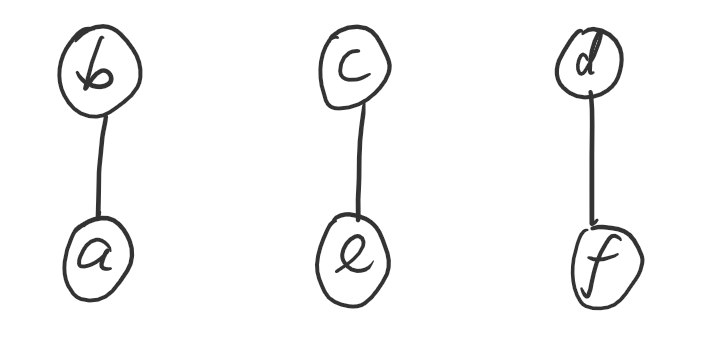
\includegraphics[width=0.7\linewidth]{ex8-1}
		\end{figure}
		\item $G_n$ can be a matching with $2n$ vertexes, as is shown below
		\[
		\begin{matrix}
		a_1&\rule[.5mm]{8mm}{.2mm}&b_1\\
		a_2&\rule[.5mm]{8mm}{.2mm}&b_2\\
		\cdots&\rule[.5mm]{8mm}{.2mm}&\cdots\\
		a_n&\rule[.5mm]{8mm}{.2mm}&b_n\\
		\end{matrix}
		\]
	\end{enumerate}
	\subsection*{4.3.2.6}
	Algorithm 4.3.2.1 will always computes an optimal vertex cover for the infinite family of stars starting from $K{2,n}$, i.e., $K_n,\ n=3,4,\cdots$
	\subsection*{4.3.2.9}
	\begin{enumerate}[(a)]
		\item 
		\begin{codebox}
			\zi\proc{Tree-Min-VCP(\id{r})}\li 
			\If \id{r}==\const{NULL}\li 
			\Then \Return 0\End\li
			\If \id{r}$\rightarrow$\id{left}==\const{NULL} and \id{root}$\rightarrow$\id{right}==NULL\li 
			\Then \Return 0\End\li 
			$\id{size\_incl}\gets 0$\li 
			\If \id{r}$\rightarrow$\id{left}\Then\li 
			\id{size\_incl}=1+\proc{Min-VCP(\id{r}$\rightarrow$\id{left}$\rightarrow$\id{left})}+\proc{Min-VCP(\id{r}$\rightarrow$\id{left}$\rightarrow$\id{right})}\End\li 
			\If \id{r}$\rightarrow$\id{right}\Then\li 
			\id{size\_excl}=1+\proc{Min-VCP(\id{r}$\rightarrow$\id{right}$\rightarrow$\id{left})}+\proc{Min-VCP(\id{r}$\rightarrow$\id{right}$\rightarrow$\id{right})}\End\li 
			\Return $\min(size\_incl, size\_excl)$
		\end{codebox}
		\item 
		\begin{codebox}
			\zi\proc{2-Approx-Min-VCP(\id{G})}\li 
			Let \id{V'} be a new empty set of vertexes\li 
			\For each edge $(\id{u},\id{v})\in G.E$\Do\li 
			\If $u\notin V'$ and $v\notin V'$\Then\li 
			$V'=V'\cup \left\{u,v\right\}$\End\End\li 
			\Return $V'$
		\end{codebox}	
	\end{enumerate}
\end{document}